%
% LaTeX report template 
%

% This is a comment: in LaTeX everything that in a line comes
% after a "%" symbol is treated as comment

\documentclass[11pt, a4paper]{article}
\usepackage{graphicx}
\usepackage{amsmath}
\usepackage{listings}
\usepackage{physics}
\newcommand{\appropto}{\mathrel{\vcenter{
  \offinterlineskip\halign{\hfill $##$\cr
    \propto\cr\noalign{\kern2pt}\sim\cr\noalign{\kern-2pt}}}}}
\usepackage{mathtools}
\title{Assignment No 5} % Title

\author{Sumanth R Hegde, EE17B032} % Author name

\date{\today} % Date for the report
\begin{document}		
		
\maketitle % Insert the title, author and d

\section*{Aim}
The aim of this assignment is to obtain the solution to potential in a region  by solving\textit{ Laplace's}  equation in $2$-dimensions.  

\section*{Numerical Solution to Laplace's equation}

Laplace's equation in 2-dimensions can  be written in Cartesian coordinates as 
\begin{equation}
\label{Eqn:1}
 \pdv[2]{\phi}{x} = \pdv[2]{\phi}{y} 
\end{equation}


An approximate solution for the above equation for a 2-dimensional grid of points would be 
\begin{equation*}
\phi_{i,j} = \frac{\phi_{i,j-1}+\phi_{i-1,j}+\phi_{i+1,j}+\phi_{i,j+1}}{4} 
\end{equation*}ie. the solution at any point is a sum of values at neighbouring points. The algorithm implemented makes use of the above equation to update $\phi$  over many iterations till it converges within an acceptable error.

\section*{The Potential Solution}
Along with the update mentioned in Eqn.\ref{Eqn:1}  we also need to take care of the boundary conditions imposed on the system. The following code blocks update the value of $\phi$ over \texttt{Niter} iterations, along with the error profile :
\begin{verbatim}
def phi_update(phi,oldphi):
    phi[1:-1,1:-1] = 0.25*(oldphi[1:-1,0:-2]+oldphi[1:-1,2:]+ 
    oldphi[0:-2,1:-1]+oldphi[2:,1:-1]) 
    return phi
 \end{verbatim}
 \begin{verbatim}
def boundary_conditions(phi,inds):
    phi[1:-1,0] = phi[1:-1,1]
    phi[0,1:-1] = phi[1,1:-1]
    phi[1:-1,-1] = phi[1:-1,-2]
    phi[-1,1:-1] = 0
    phi[inds] = 1.0
    return phi
\end{verbatim}
\begin{verbatim}
for i in range(Niter):
    oldphi = phi.copy()
    phi = phi_update(phi,oldphi)
    phi = boundary_conditions(phi,inds)
    error[i] = (abs(phi-oldphi)).max()
\end{verbatim}

The initial potential configuration of the system can be visualised using the \texttt{pylab.contourf()} function :

\begin{verbatim}
pylab.contourf(range(Nx),range(Ny),phi.T,cmap=pylab.cm.get_cmap("autumn"))
pylab.xlabel(r'x$\rightarrow$',fontsize=15)
pylab.ylabel(r'y$\rightarrow$',fontsize=15)
\end{verbatim}

\begin{figure}[!htb]
\centering
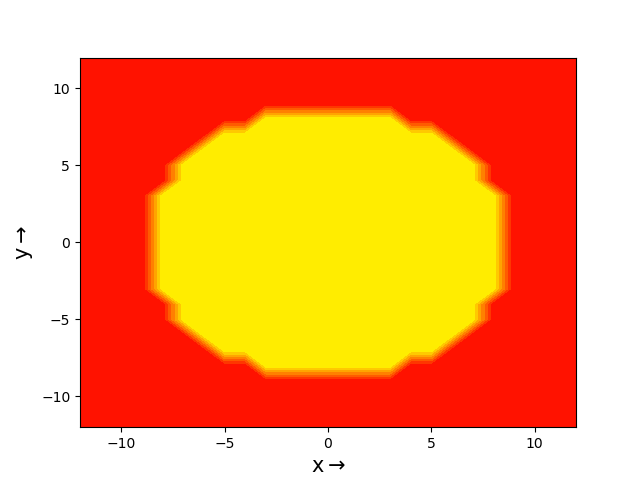
\includegraphics[scale=0.5]{potential.png}
\caption{Plot of the initial potential configuration}
\label{fig:1}
\end{figure}

\newpage

\section*{Error in estimation}

The evolution of the error with the number of iterations is 

\begin{figure}[!htb]
\centering
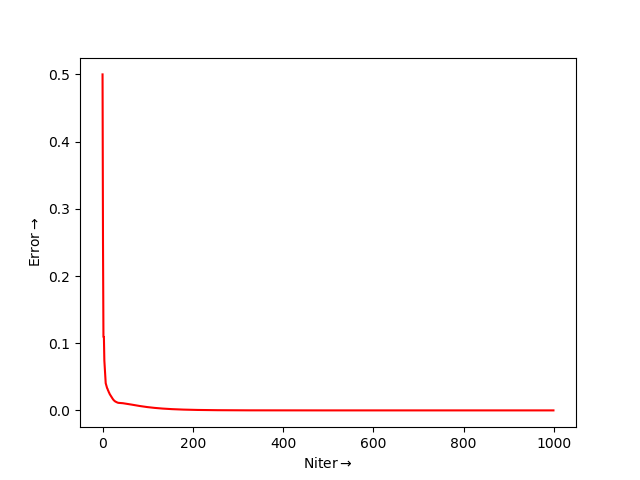
\includegraphics[scale=0.5]{Error.png}
\caption{Error vs \textit{Niter}}
\label{fig:3}
\end{figure}

Using a semilog plot, and considering only every 50th point for the sake of better visualization, we obtain the following plot :
\begin{figure}[!htb]
\centering
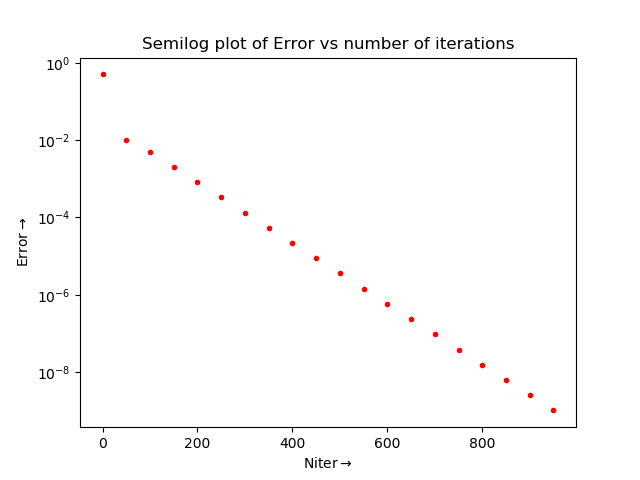
\includegraphics[scale=0.5]{semilog1.png}
\caption{Semilog plot of Error vs number of iterations}
\label{fig:4}
\end{figure}
\newpage
Similarly, the following is the loglog plot :
\begin{figure}[!htb]
\centering
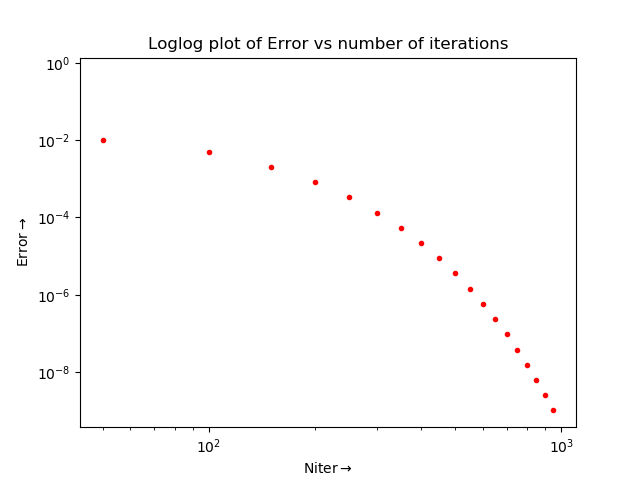
\includegraphics[scale=0.4]{loglog1.png}
\caption{Loglog plot of Error vs number of iterations}
\label{fig:5}
\end{figure}
 
The error function appears to vary exponentially with \textit{Niter}. We attempt to extract the exponent of this dependence.  In  particular, we attempt to fit a function of the form
\begin{equation*}
y = Ae^{Bx}
\end{equation*}
Thus ,
\begin{equation*}
logy = logA + Bx
\end{equation*}
$logA$ and $B$ can be estimated using the least squares method. The following code block accomplishes the same :
\begin{verbatim}
def error_fit(x,y):
    logy=np.log(y)
    xvec=np.zeros((len(x),2))
    xvec[:,0]=x
    xvec[:,1]=1
    B,logA=np.linalg.lstsq(xvec, np.transpose(logy))[0]
    return (np.exp(logA),B)
\end{verbatim}
The parameters $A$ and $B$ are obtained in two ways : 
\begin{itemize}
\item Fitting the entire error vector ( \textit{fit1} )
\item Fitting only the points beyond 500 iterations( \textit{fit2} )
\\
\newpage
The fit in both cases when plotted with the original error function yield the following graph : 
\end{itemize}
  \begin{figure}[!h]
 \centering
 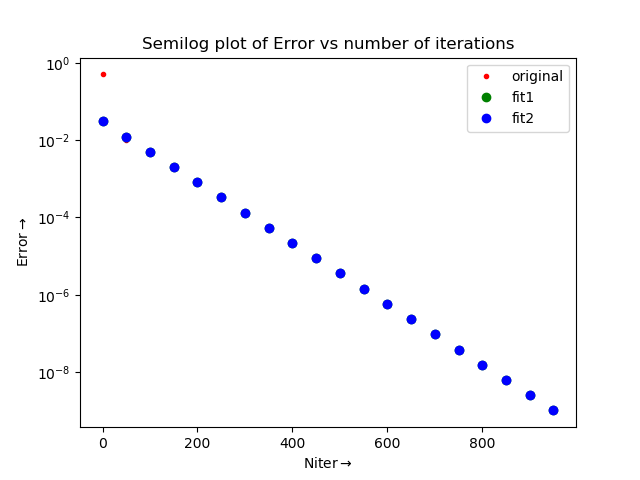
\includegraphics[scale=0.4]{semilog2.png}
 \caption{Semilog plot of Error vs number of iterations}
 \end{figure}
 
 Notice that the plots almost exactly coincide, with differences hardly visible. 
 
\section*{Stopping condition }
The upper bound for the error estimated with each iteration is given by \\
\begin{center}
Error = $-\dfrac{A}{B} exp(B(N+0.5))$ 
\end{center}

This can be plotted with the number of iterations \textit{Niter} . The following graph is obtained  :
\begin{figure}[!h]
\centering
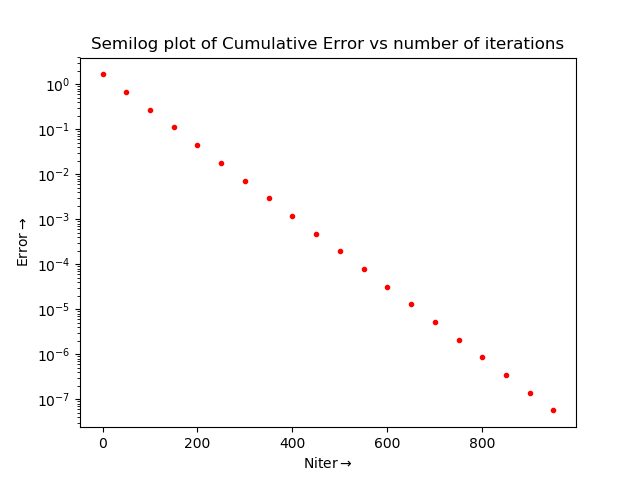
\includegraphics[scale=0.4]{Cumulative_error.png}
\caption{}
\end{figure}

\section*{Surface plot of potential}
After running the update for 1000 iterations, we obtain the following 3-D plot for the potential using the \texttt{plot\_surface} function :  

\begin{figure}[!htb]
\centering
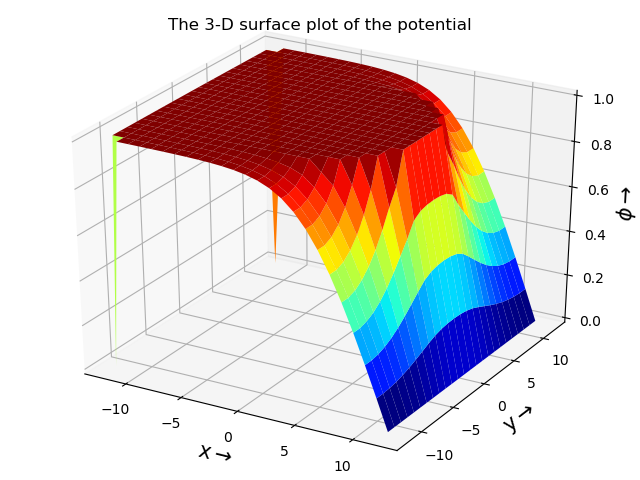
\includegraphics[scale=0.5]{3-d.png}
\caption{3-D surface plot of $\phi$  after \textit{1000} iterations}
\label{fig:2}
\end{figure}

The contour plot of $\phi$ is obtained using the \texttt{pylab.contour} function. 
   \begin{figure}[!h]
 \centering
 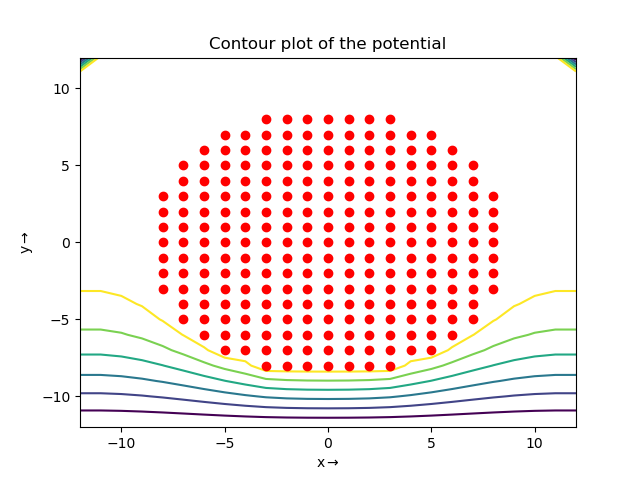
\includegraphics[scale=0.5]{contour.png}
 \caption{Contour plot of $\phi$}
 \end{figure}
 \newpage
 
 \section*{Vector plot of Currents}
 
 The currents in the system in Cartesian form can be expressed as :
 \begin{equation*}
 J_{x} = - \pdv{\phi}{x}  
 \end{equation*}
\begin{equation*}
  J_{y} = - \pdv{\phi}{y} 
 \end{equation*}
 
 Numerically, this can be expressed as 
 \begin{equation*}
   J_{x,ij} = \frac{\phi_{i,j+1}-\phi_{i,j-1}}{2}
 \end{equation*} \begin{equation*}
   J_{y,ij} = \frac{\phi_{i+1,j}-\phi_{i-1,j}}{2}
 \end{equation*}The following code block evaluates the currents $J_x$ and $J_y$ :
 \begin{verbatim}
     Jx = np.zeros((Ny,Nx))
     Jy = np.zeros((Ny,Nx))
     Jx[:,1:-1] = 0.5*(potential[:,0:-2]-potential[:,2:])
     Jy[1:-1] = 0.5*(potential[2:, :]-potential[0:-2,:])
 \end{verbatim}
 The current density vector is now plotted using the \texttt{quiver}  function. The following plot is obtained :
 
  \begin{figure}[!h]
 \centering
 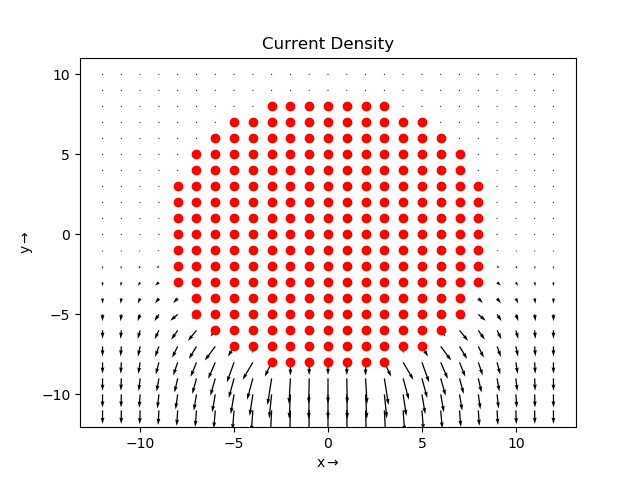
\includegraphics[scale=0.5]{current.png}
 \caption{Current density profile}
 \end{figure}
 


From the current density plot, we notice that hardly any current flows through the top part of the wire. With a little thought, we observe that the lower surface being grounded, the easiest way for charge carriers to flow from the electrode would be directly through the lower half of the wire, thus avoiding a longer,  more resistive path through the top half of the wire.

\section*{ Conclusion}
Using a finite differentiation approximation, we have found a solution to Laplace's equation for a given system. The error is seen to decay at a highly gradual pace. Thus the chosen method of solving Laplace's equation is inefficient.  On analysing the quiver plot of the currents, it was noticed that the current was mostly restricted to the bottom of the wire, and was perpendicular to the surface of the electrode and the conductor. 
\end{document}



